\documentclass{standalone}

\usepackage{fontspec}
%\setmainfont{VT323}


\usepackage[dvipsnames]{xcolor}
\usepackage{tikz}
\usetikzlibrary{shapes.geometric}

\tikzset{cross/.pic={
\path[draw, thick, fill=white] (0,10mm) -- (3mm, 10mm) -- (3mm,3mm) -- (10mm,3mm) -- (10mm,-3mm) -- (3mm,-3mm) -- (3mm,-10mm) -- (-3mm, -10mm) -- (-3mm, -3mm) -- (-10mm, -3mm) -- (-10mm, 3mm) -- (-3mm,3mm) -- (-3mm, 10mm) -- cycle;
}}

%\pagecolor{yellow!50}
\begin{document}
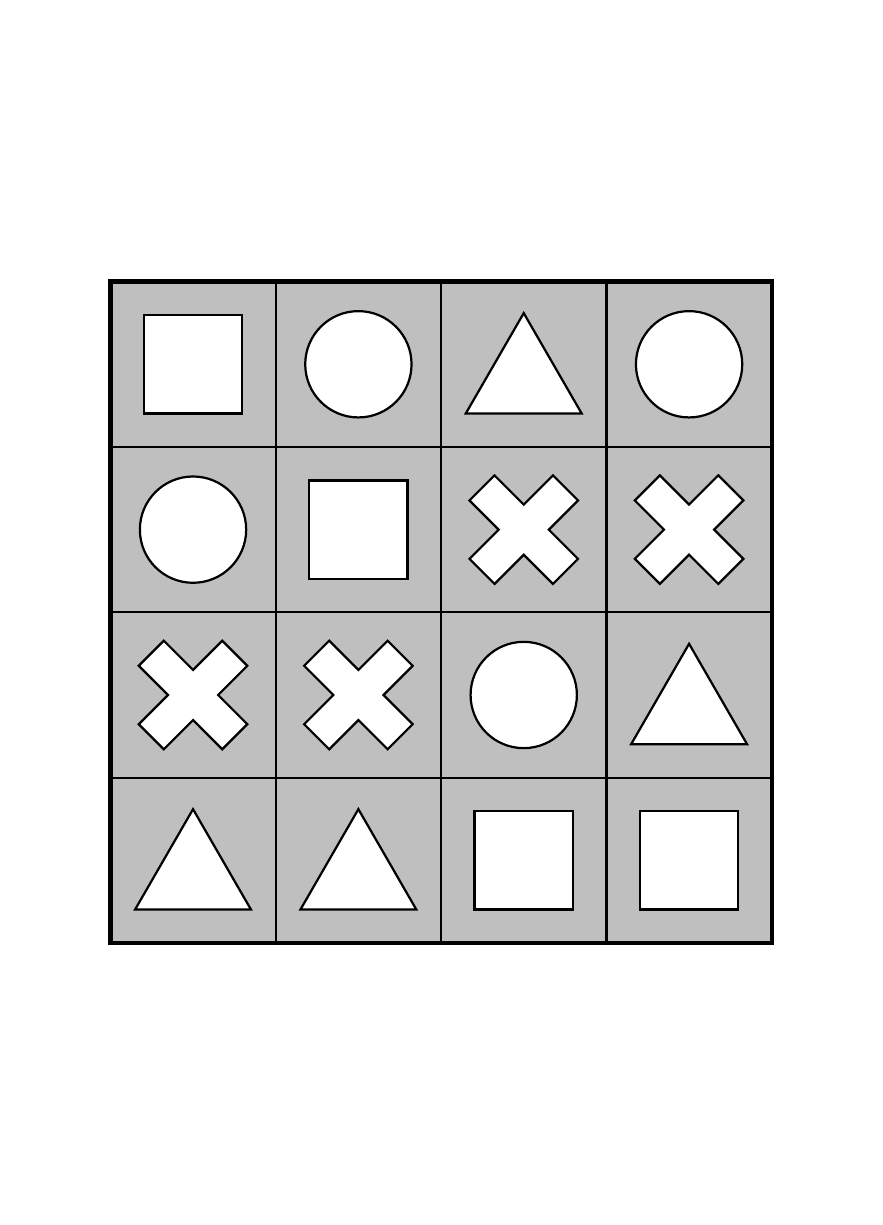
\begin{tikzpicture}
\path (-52.5mm, -74.25mm) -- (52.5mm, 74.25mm);
\node[inner sep=0pt, minimum width=84mm, minimum height=84mm, draw, ultra thick, fill=lightgray] at (0,0) {};

\foreach \x in {-31.5mm, -10.5mm, 10.5mm, 31.5mm}
	\foreach \y in {-31.5mm, -10.5mm, 10.5mm, 31.5mm}
		\node[draw, thick, minimum width=21mm, minimum height=21mm] at (\x, \y) {};
		
\node[draw, thick, fill=white, minimum width=12.5mm, minimum height=12.5mm] at (-31.5mm, 31.5mm) {};
\node[draw, thick, fill=white, minimum width=12.5mm, minimum height=12.5mm] at (-10.5mm, 10.5mm) {};
\node[draw, thick, fill=white, minimum width=12.5mm, minimum height=12.5mm] at (10.5mm, -31.5mm) {};
\node[draw, thick, fill=white, minimum width=12.5mm, minimum height=12.5mm] at (31.5mm, -31.5mm) {};

\node[draw, thick, fill=white, circle, minimum width=13.5mm] at (-10.5mm, 31.5mm) {};
\node[draw, thick, fill=white, circle, minimum width=13.5mm] at (31.5mm, 31.5mm) {};
\node[draw, thick, fill=white, circle, minimum width=13.5mm] at (-31.5mm, 10.5mm) {};
\node[draw, thick, fill=white, circle, minimum width=13.5mm] at (10.5mm, -10.5mm) {};

\node[draw, thick, fill=white, regular polygon, regular polygon sides=3, minimum width=17mm] at (10.5mm, 29.5mm) {};
\node[draw, thick, fill=white, regular polygon, regular polygon sides=3, minimum width=17mm] at (31.5mm, -12.5mm) {};
\node[draw, thick, fill=white, regular polygon, regular polygon sides=3, minimum width=17mm] at (-31.5mm, -33.5mm) {};
\node[draw, thick, fill=white, regular polygon, regular polygon sides=3, minimum width=17mm] at (-10.5mm, -33.5mm) {};

\pic[rotate=45, scale=0.75] at (10.5mm, 10.5mm) {cross};
\pic[rotate=45, scale=0.75] at (31.5mm, 10.5mm) {cross};
\pic[rotate=45, scale=0.75] at (-31.5mm, -10.5mm) {cross};
\pic[rotate=45, scale=0.75] at (-10.5mm, -10.5mm) {cross};


\end{tikzpicture}
\end{document}